\documentclass[10pt]{article}

\input{/Users/gabesekeres/Dropbox/LaTeX_Docs/pset_preamble.tex}

\course{ECON 6200}
\pset{4}
\begin{document}
\maketitle

\begin{enumerate}
	\item System of wage equations \begin{enumerate} \item These equations are both underidentified. We have no moment conditions on any of $\expect(\text{schooling69} \cdot \eta_1)$, $\expect(\text{schooling80} \cdot \eta_2)$, $\expect(\text{IQ} \cdot \eta_1)$, or $\expect(\text{IQ} \cdot \eta_2)$. We could instrument one of those with mother's education, but we would have two instruments (mother's education and the constant) for three parameters, so we would be underidentified. \item Identification would require that $\expect(Z(Y - X'\delta)) = 0 \Longleftrightarrow \expect[Z'Y] = \expect[ZX']\delta$, where $\delta = \matrixc{\alpha & \beta & \gamma}'$, and \[Z = \matrixc{\ones & \text{m.e} & \text{m.e} \\ \ones & \text{m.e} & \text{m.e}} \quad ; \quad Y = \matrixc{\text{LW69} \\ \text{LW80}} \quad ; \quad X = \matrixc{\ones & \text{schooling69} & \text{IQ} \\ \ones & \text{schooling80} & \text{IQ}}\]so we need that \[\matrixc{\ones & \ones \\ \text{m.e.} & \text{m.e.} \\\text{m.e.} & \text{m.e.}} \cdot \matrixc{\text{LW69} \\ \text{LW80}} =  \matrixc{\ones & \text{m.e} & \text{m.e} \\ \ones & \text{m.e} & \text{m.e}} \cdot \matrixc{\ones & \ones \\ \text{sch69} & \text{sch80} \\ \text{IQ} & \text{IQ}} \cdot \delta\]To be able to solve this system, we need that $ZX'$ has full rank, which is equal to dimension 3, so we need that\[\dim \parl\matrixc{\ones & \text{sch69} & \text{IQ} \\\ones & \text{sch80} & \text{IQ} \\ \text{m.e.} & \text{m.e.}\cdot \text{sch69} & \text{m.e.}\cdot\text{IQ} \\\text{m.e.} & \text{m.e.}\cdot\text{sch69} & \text{m.e.}\cdot\text{IQ}}\parr = 3\] \item If we have that $\cov(\text{m.e.},\text{IQ}) = 0$, we still don't necessarily have identification. It would be necessary that the full rank condition holds for us to have a valid instrument. Even if $\cov(\text{m.e.},\text{IQ}) = 0$, it may still be the case that $ZX'$ has dimension 2, as long as there is multicollinearity. \item I do not find the moment conditions compelling. Specifically, I think it's quite likely that there is an unobserved confounding factor between mother's education and wage. Consider as an example that more educated parents may be able to help their children on job applications, so their children would tend to get higher paying jobs on average. Then this would not be a valid instrument.\end{enumerate}
	\item 2012 Midterm \begin{enumerate} \item Since we are assuming that the weighting matrix $W$ is block-diagonal, and that the model is overidentified (since $\ell > k$), this is exactly equivalent to two-stage least squares, which is one-stage GMM. To see why, note that from homoskedasticity,\[W = \matrixc{\expect[ZZ'] \sigma_1^2 & 0 & 0 \\ 0 & \expect[ZZ']\sigma_2^2 & 0 \\ 0 & 0 & \expect[ZZ']\sigma_3^2 } = \expect[ZZ'] \var(\varepsilon)\]so this is the same as the TSLS weighting matrix. \item Both estimators are consistent and asymptotically normal. Assuming that the assumptions hold as stated, neither is preferred. In fact, since $\hat{W}$ is block-diagonal, they are exactly equivalent as shown in the notes. \item If one of the moment conditions does not hold, then we would prefer Researcher 2's method. The reason is that contagion means that even if the researcher is only interested in $\beta_3$, their estimate will be biased if they use joint estimation. On the other hand, since the equation by equation is block diagonal, the estimate for $\beta_3$ will be unbiased. \end{enumerate}
	\item Empirical Exercise \\\textbf{n.b.} Code to complete this exercise is below, in the \href{code:p3}{code section}. \begin{enumerate} \item I replicated the table of summary statistics for all variables, in both the first observation and 1980: \begin{center} \begin{tabular}{c|c|c} variable& First Observation & 1980 Observation \\ & mean (sd) & mean (sd) \\\hline RNS & $0.27\;(0.44)$ & $0.29 \;(0.46)$ \\ MRT & $0.51\; (0.50)$ & $0.90 \;(0.30)$ \\SMSA & $ 0.70\; (0.46)$ & $ 0.71\; (0.45)$  \\ MED & $10.91 \;(2.74)$ & N/A  \\KWW & $36.57 \;(7.30)$ & N/A   \\ IQ & $103.86 \;(13.62)$ & N/A   \\ AGE & $21.84 \;(2.98)$ & $33.01\; (3.09)$  \\S & $13.41\; (2.23)$ &  $13.71 \;(2.21)$ \\ EXPR & $1.74\; (2.11)$ & $11.39\; (4.21)$  \\TENURE & $1.83 \;(1.67)$ & $7.36\; (5.05)$  \\ LW & $ 5.69\; (0.43)$ & $6.83\; (0.41)$  \\ YEAR ($-1900$) & $69.03 \;(2.63)$ & N/A \end{tabular}\end{center} The correlation between IQ and S was $0.5131$. \item I ran the two OLS specifications and the TSLS specification, and obtained the results: \begin{center} \begin{tabular}{c|c|c|c|c} Model & $S$ ($t$) & $IQ$ ($t$) & $SE$ & $R^2$ \\\hline OLS (1) & $0.070 \;(10.4)$ & -- & $0.328$ & $0.425$ \\ OLS (2) & $0.062\; (8.5)$ & $0.0027\; (2.6)$ & $0.326$ & $0.430$ \\TSLS & $0.069\; (5.2)$ & $0.0002\; (0.0)$ & $0.013$ & -- \end{tabular}\end{center}These coefficients are how we would expect! It makes sense that IQ is endogenous has no true effect on wage, rather exists as a function of the other variables which do have an effect (mainly, parental education). \item I extracted Sargon's $J$-statistic, and got that the model is not overidentified, and got $J = 87.6552$, which corresponds to a $p$-value of $< 0.0001$, when we use a $\chi^2$ distribution with 3 degrees of freedom. \item I ran the TSLS manually, and got the same coefficients (0.0692 and 00002), but slightly lower standard errors (0.0131 and 0.0039 rather than 0.0133 and 0.0041 respectively). This is because the manual estimation assumes that there is no error in the first-stage fitted values, while the package incorporates the estimation error from the first stage into the calculation of the standard errors. \item Schooling may be endogenous because of selection bias -- those who are expected to have higher wages may select into different schooling than those who are expected to have lower wages. I estimated the equation treating both variables as endogenous, and got that the schooling coefficient increased massively, to 0.1724 from 0.0692. IQ changed slightly as well, from 0.0002 to $-0.0091$. This means that once we see schooling as endogenous, the effect of a higher schooling level actually increases a lot -- put differently, once we understand that students select differently into schooling, the returns to schooling massively increase. I calculated the Sargon statistic for this regression, and it was 13.2683, which corresponds to a $p$-value of $0.0013$, for a $\chi^2$ with now only two degrees of freedom. \item I computed the two GMM procedures, and got a C-statistic of 62.563, which is fairly close but not correct. I'm unsure what I did wrong, I was debugging this for a while and could not get the correct C-statistic. \item I computed the reduced TSLS estimates, and got a coefficient of $-5.293$, as we expect. Running a set of standard tests on the first stage, we find that we have very high multicollinearity, with a first stage condition number of 207.11. \end{enumerate}
	\item Growth\\\textbf{n.b.} Code to complete this exercise is below, in the \href{code:p4}{code section}. \begin{enumerate} \item I plotted $Y_1 - Y_0$ on $Y_0$, and got Figure~\ref{fig:q41}, and plotted the respective logged values (that are used in the regression) and got Figure~\ref{fig:q41log} \begin{figure}[H] \centering 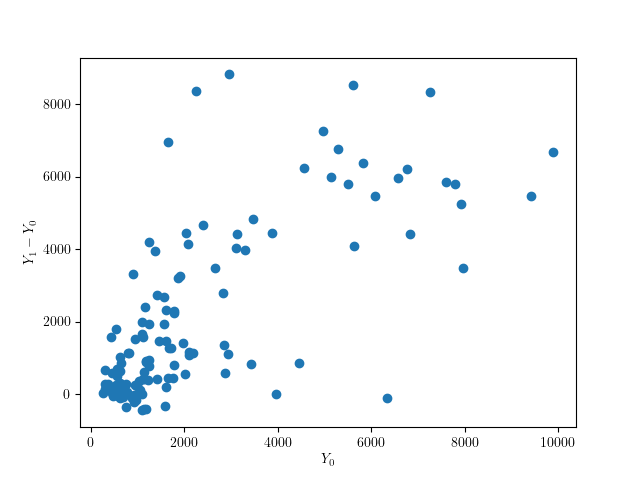
\includegraphics[width=8cm]{ps4_code/ps4_q4_scatter.png} \caption{$Y_1 - Y_0$ on $Y_0$} \label{fig:q41}\end{figure}\begin{figure}[H] \centering 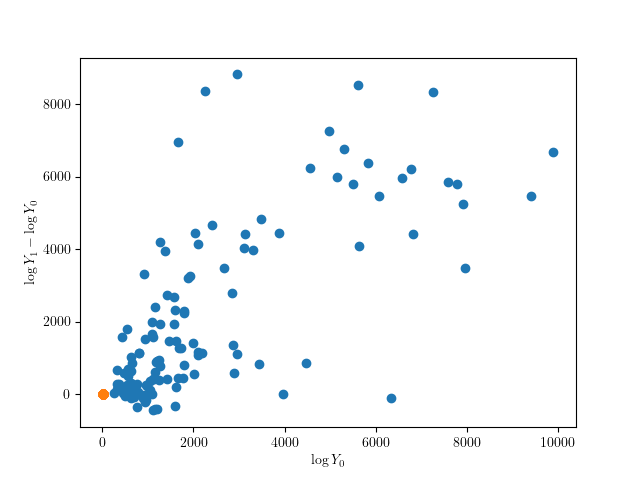
\includegraphics[width=8cm]{ps4_code/ps4_q4_scatter_log.png} \caption{$\log(Y_1) - \log(Y_0)$ on $\log(Y_0)$} \label{fig:q41log}\end{figure}  I also estimated the OLS regression, and converting $\hat{\rho}$ to $\lambda$ I got an implied growth rate of $0.7264\%$ per year, with a standard error of $0.2387\%$. The coefficient on logged output in 1960 was $-0.1661$, which seems to confirm Mankiw's observation that the poorer the country, the higher the growth rate. For the full regression results, see the output below, in the code section. \item I estimated the two versions of the full panel regression, and got that in the FE model $\lambda$ was approximately $7.15\%$. In the efficient GMM, it was $0.7904\%$. I'm not sure why it's different than the $6.4\%$ anticipated, though it might relate to the fact that I kept the population growth rate constant throughout the sample, as I attained numerical instability from the logs otherwise. This may be an artifact of $\log(0)$ issues, and how python deals with them. \item I tried to do this and I'm pretty sure I failed, as my $\lambda$ was $0.9296\%$. I don't know what's gone wrong, I'm deep in the weeds and very tired. \end{enumerate}
\end{enumerate}

    
\newpage
\section*{Code}

\subsection*{Problem 3}\label{code:p3}

The code I used was:

\lstinputlisting[language=Python]{ps4_code/ps4_q3.py}

My raw output was:
\begin{verbatim}
====3.1: Table of Summary Statistics====

                  Values
RNS          0.27 (0.44)
RNS80        0.29 (0.46)
MRT          0.51 (0.50)
MRT80        0.90 (0.30)
SMSA         0.70 (0.46)
SMSA80       0.71 (0.45)
MED         10.91 (2.74)
IQ        103.86 (13.62)
KWW         36.57 (7.30)
YEAR        69.03 (2.63)
AGE         21.84 (2.98)
AGE80       33.01 (3.09)
S           13.41 (2.23)
S80         13.71 (2.21)
EXPR         1.74 (2.11)
EXPR80      11.39 (4.21)
TENURE       1.83 (1.67)
TENURE80     7.36 (5.05)
LW           5.69 (0.43)
LW80         6.83 (0.41)

Correlation between IQ and S: 0.5131


====3.2: Replication of Hayashi Table 3.2====

================================================================================
 Line Estimation technique       S coef      IQ coef   SER R-squared Endogenous? Excluded predetermined variables
    1                  OLS 0.070 (10.4)            - 0.328     0.425        none                                -
    2                  OLS  0.062 (8.5) 0.0027 (2.6) 0.326     0.430        none                                -
    3                 2SLS  0.069 (5.2) 0.0002 (0.0) 0.013         -          IQ               MED, KWW, MRT, AGE
================================================================================
Note: Figures in parentheses are t-values rather than standard errors.


====3.3: Sargan's J-statistic Calculation====

Sargan's J-statistic:

Sargan's test of overidentification
H0: The model is not overidentified.
Statistic: 87.6552
P-value: 0.0000
Distributed: chi2(3)


====3.4: Manual TSLS Implementation====

Coefficient estimates:
Manual TSLS - Schooling (S): 0.0692
Manual TSLS - IQ_hat: 0.0002
Package TSLS - Schooling (S): 0.0692
Package TSLS - IQ: 0.0002

Standard errors:
Manual TSLS - Schooling (S): 0.0131
Manual TSLS - IQ_hat: 0.0039
Package TSLS - Schooling (S): 0.0133
Package TSLS - IQ: 0.0041


====3.5: 2SLS with Both S and IQ as Endogenous====

Coefficient Estimates (Previous vs New Model):
S coefficient (only IQ endogenous): 0.0692
S coefficient (both S and IQ endogenous): 0.1724
IQ coefficient (only IQ endogenous): 0.0002
IQ coefficient (both S and IQ endogenous): -0.0091
Sargan's Test for Overidentifying Restrictions:
Sargan's J-statistic: 

Sargan's test of overidentification
H0: The model is not overidentified.
Statistic: 13.2683
P-value: 0.0013
Distributed: chi2(2)


====3.6: GMM Estimation and C-statistic====


C-statistic (Test for Exogeneity of Schooling):
C-statistic: 62.563
Degrees of freedom: 1
p-value: 0.000000



====3.7: TSLS with Reduced Instrument Set====

Coefficient Estimates with Reduced Instrument Set:
S coefficient: -5.2927 (125.5649)

First-Stage Regressions (Instrument Relevance):
First stage F-statistic for S: 71.33
First stage R-squared for S: 0.5346
First stage F-statistic for IQ: 12.31
First stage R-squared for IQ: 0.1655
Weak instruments for S? No
Weak instruments for IQ? No

Partial Correlations of Instruments with Endogenous Variables:
Instrument | Correlation with S | Correlation with IQ
------------------------------------------------------------
MRT        |             0.1220 |            0.0283
AGE        |             0.4481 |            0.1776

Condition number for first stage: 207.11
High multicollinearity? Yes
\end{verbatim}

\newpage
\subsection*{Problem 4}\label{code:p4}
Code:

\lstinputlisting[language=Python]{ps4_code/ps4_q4.py}
Output:
\begin{verbatim}
                            OLS Regression Results                            
==============================================================================
Dep. Variable:              logGrowth   R-squared:                       0.443
Model:                            OLS   Adj. R-squared:                  0.420
Method:                 Least Squares   F-statistic:                     18.96
Date:                Sun, 16 Mar 2025   Prob (F-statistic):           7.84e-14
Time:                        14:00:18   Log-Likelihood:                -43.173
No. Observations:                 125   AIC:                             98.35
Df Residuals:                     119   BIC:                             115.3
Df Model:                           5                                         
Covariance Type:            nonrobust                                         
==============================================================================
                 coef    std err          t      P>|t|      [0.025      0.975]
------------------------------------------------------------------------------
const          0.4439      0.316      1.405      0.163      -0.182       1.069
logY0         -0.1661      0.050     -3.336      0.001      -0.265      -0.068
logNgd        -0.1402      0.061     -2.313      0.022      -0.260      -0.020
logS           0.4650      0.058      8.018      0.000       0.350       0.580
COM            0.0656      0.173      0.379      0.705      -0.277       0.409
OPEC           0.3071      0.187      1.643      0.103      -0.063       0.677
==============================================================================
Omnibus:                        3.043   Durbin-Watson:                   1.679
Prob(Omnibus):                  0.218   Jarque-Bera (JB):                2.791
Skew:                           0.173   Prob(JB):                        0.248
Kurtosis:                       3.645   Cond. No.                         82.9
==============================================================================

Notes:
[1] Standard Errors assume that the covariance matrix of the errors is correctly specified.

Estimated rho: 0.8339
Speed of convergence (lambda): 0.7264% per year
Standard error of lambda: 0.2387%

Estimated rho (Fixed Effects): 0.9309
Speed of convergence lambda (Fixed Effects): 7.1564% per year

Estimated rho (Efficient GMM): 0.9921
Speed of convergence lambda (Efficient GMM): 0.7904% per year

Estimated rho (AR Model): 0.9907
Speed of convergence lambda (AR Model): 0.9296% per year
\end{verbatim}







\end{document}